\documentclass[12pt,a4paper]{article}
    \usepackage[utf8]{inputenc}
    \usepackage{amsmath}
    \usepackage{amsfonts}
    \usepackage{amssymb}
    \usepackage[danish]{babel}
    \usepackage{graphicx}
    \usepackage{natbib}
    \usepackage{siunitx}
    \usepackage{fancyhdr}
    \usepackage{adjustbox}%Gør det muligt at have en "tabel" der kan gå ud over begge marign, istedet for kun den ene (højre)
    \usepackage{titling} %Package som bruges til at fjerne number på forside.

% Vandmærke
    %\usepackage{draftwatermark}
    %\SetWatermarkText{
\includegraphics{fig/dtu/dtu-logo-3.png}}
% Udvidet side hoved/fod
    \pagestyle{fancy}
    \fancyhf{}
    \fancyfoot[RE,RO]{
\includegraphics[height=4.5cm]{fig/dtu/dtu.png}}
% lstlisting - til brug ved indsættelse af kode
\usepackage{listings}
\usepackage{color}

\definecolor{dkgreen}{rgb}{0,0.6,0}
\definecolor{gray}{rgb}{0.5,0.5,0.5}
\definecolor{mauve}{rgb}{0.58,0,0.82}

\lstset{frame=tb,
  language=Java,
  aboveskip=1.5mm,
  belowskip=1.5mm,
  showstringspaces=false,
  columns=flexible,
  basicstyle={\small\ttfamily},
  numbers=none,
  numberstyle=\tiny\color{gray},
  keywordstyle=\color{blue},
  commentstyle=\color{dkgreen},
  stringstyle=\color{mauve},
  breaklines=true,
  breakatwhitespace=true,
  tabsize=3
}
% Hyperlinks
\usepackage{hyperref}
\usepackage{color}


\title{CDIO2}
\author{Gruppe 16}
\date{10. november 2017}

% Sidehoved
    \pagestyle{fancy}
    \lhead{Gruppe 16}
    \rhead{02313 - 02315}
    \chead{CDIO2}


    \author{Gruppe 16}
    \title{CDIO3}
    \pagestyle{fancy}
    \lhead{Gruppe 16}
    \rhead{CDIO3}
    \chead{1. december 2017}


    \begin{document}
          \begin{titlingpage}
        %Dette er vores forside
        \maketitle %Dette er toppen
        % Her er navn og billeder:
        \begin{adjustbox}{center}
                \begin{tabular}{llllll}
                     
\includegraphics[height=3cm]{fig/gruppeBilleder/mfager.png} &  
\includegraphics[height=3cm]{fig/gruppeBilleder/milishia.png} &
                     
\includegraphics[height=3cm]{fig/gruppeBilleder/nicki.png} &
                     
\includegraphics[height=3cm]{fig/gruppeBilleder/semi.png} &
                     
\includegraphics[height=3cm]{fig/gruppeBilleder/simon.png} &
                     
\includegraphics[height=3cm]{fig/gruppeBilleder/thyge.png}
                \\ % Næste række
                     Mathias & Milishia & Nicki & Semi & Simon & Thyge
                \\
                Fager & Moardi & Christiansen & Seitovski & Pedersen & S. Steffensen
                \\
                s175182 & s175193 & s170208 & s175181 & s175195 &s175176
                \end{tabular}
                
                \label{tab:my_label}
        \end{adjustbox}
        \vspace{.5cm}
        \begin{center}
            
\includegraphics{fig/dtu/DTU_small.png}
        \end{center}
    \end{titlingpage}
        \pagebreak
        \section*{Timeregnskab}
Timeregnskabet kan ses via linket 
    \color{blue}
    \underline{\href{https://goo.gl/Rsx9wG}{her}}
    \color{black}
 eller i billag XX.

 %------------------------------------------------------------------------------------
 %                              Indholdsfortegnelse
 %------------------------------------------------------------------------------------
\pagebreak
\tableofcontents

        \pagebreak
        \section{Analyse}
        
    
    \subsection{Kravliste}
        \begin{enumerate}
<<<<<<< HEAD
<<<<<<< HEAD
<<<<<<< HEAD
            \item Spillet skal være mellem 2 - 4 personer
            \item Spillerne skal slå terninger på skift
            \item Der skal udskrives en tekst der omhandler det aktuelle felt, når spilleren lander på et felt
            \item Hver felt skal have en effekt for spilleren
            \item Spillerne starter med en balance på:
            \begin{enumerate}
                \item 20, hvis der er 4 spillere.
                \item 18, hvis der er 3 spillere.
                \item 16, hvis der er 2 spillere.
            \end{enumerate}
            %Efter de nye regler så starter spillerne med hhv. 20, 18 eller 16 Matadollars, alt efter om der er 2, 3 eller 4 spillere.
            \item Spillet slutter når den første spiller har mistet alle sine penge.
            %Efter de nye regler så er der når den første spille går bankerot
            \item Spillerne skal kunne gå flere omgange rundt på spillepladen.
            \item Spillet skal kunne køre på DTU’s databarer.
        \end{enumerate}

%---------------------------------------------------------------------------
%                             Input af usecases
%--------------------------------------------------------------------------
\input{UseCases.tex}

<<<<<<< HEAD
\subsection{UseCases}
%1. UseCase
\begin{center}
\begin{tabular}{ | m{10em} | m{10cm}| }
        \hline
            UseCase Section: Opsætning af spil & Comment\\
        \hline
            Scope & Monopoly spil af IOOuterActive\\
        \hline
            Level & User-goal\\
        \hline
            Primær Aktør & Spillerne\\
        \hline
            Stakeholder og interessenter & Spillerne er interesserede i at kunne starte spillet ved at vælge antal spillere og deres brikker\\
        \hline
            Forudsætninger & Spillet bliver kørt, og spillerne har nu mulighed for at vælge antal spillere og ønskede brikker\\
        \hline
            Success guaranti & Der er blevet valgt antallet af spillere, og hver spiller har valgt sin brik, herefter er spillet klar til at blive spillet\\
        \hline
    \end{tabular}
\end{center}
%2. UseCase
\pagebreak
Fully dressed UseCase:
\begin{center}
\begin{tabular}{ | m{10em} | m{10cm}| }
        \hline
            UseCase Section: Spillerne slår med terningerne & Comment\\
        \hline
            Scope & Monopoly spil af IOOuterActive\\
        \hline
            Level & User-goal\\
        \hline
            Primær Aktør & Spillerne\\
        \hline
            Stakeholder og interessenter & Spillerne er interesseret i at kunne trykke på en knap, og få et billede af to terninger med tilfældige værdier\\
        \hline
            Forudsætninger & Spillet er startet op, og spillerne har valgt antallet spillere og deres ønskede brikker\\
        \hline
            Success guaranti & Der er blevet valgt antallet af spillere, og hver spiller har valgt sit navn, herefter er spillet klar til at blive spillet\\
        \hline
            Hoved succes scenarie & Spillerne får udgivet en værdi af to terninger, og lander derefter på et felt\\
        \hline
            Alternative udfald & Negative udfald:\\
                & -	IOOuterActive har opdateret spillet, og derved opstår der en fejl når spillerne slå med terningerne, der kan ende i at der ikke bliver slået to terninger\\
                & -	Systemet blokerer for en spillers tur\\
                & -	En spiller hopper fra/på, og derved skal spillet startes om\\
        \hline
            Specielle krav
            & -	Enheden som spillet kører på skal være kompatibel med Java\\
            & -	Spillerne skal kunne interagere med GUI’en ved brug af mus eller touch\\
            & -	Der skal være plads på enheden til at kunne hente spillet\\
        \hline
            Hyppighed & Hver tur bliver der slået med terninger\\
        \hline
    \end{tabular}
\end{center}

%3. UseCase
\begin{center}
\begin{tabular}{ | m{10em} | m{10cm}| }
        \hline
            UseCase Section: Spiller lander på et felt & Comment\\
        \hline
            Scope & Monopoly spil af IOOuterActive\\
        \hline
            Level & User-goal\\
        \hline
            Primær Aktør & Spillerne\\
        \hline
            Stakeholder og interessenter & Spillerne er interesseret hvilken effekt de kommer i møde når de lander på et felt\\
            Hvis feltet ikke er opkøbt af nogen, kan spilleren der er landet på feltet købe det, medmindre det er et specielt felt\\
            Hvis feltet er ejet af nogen, skal spilleren der er landet på feltet betale den der ejer feltet\\
            Feltet de lander på kan også være et fængsel, der gør at spilleren mister en tur 
        \hline
            Forudsætninger & Spillet er i gang og en spiller har slået med terningerne\\
        \hline
            Success guaranti & Spilleren køber og ejer nu feltet\\
        \hline
    \end{tabular}
\end{center}

%4. UseCase
\begin{center}
\begin{tabular}{ | m{10em} | m{10cm}| }
        \hline
            UseCase Section: Spiller trækker et chancekort & Comment\\
        \hline
            Scope & Monopoly spil af IOOuterActive\\
        \hline
            Level & User-goal\\
        \hline
            Primær Aktør & Spillerne\\
        \hline
            Stakeholder og interessenter & Spillerne er interesseret i hvilken bonus de får når de trækker et chancekort\\
        \hline
            Forudsætninger & Spillet er i gang og en spiller trækker et chancekort\\
        \hline
            Success guaranti & En spiller lander trækker et chancekort og får en belønning eller en straf\\
        \hline
    \end{tabular}
\end{center}

%5. UseCase
\begin{center}
\begin{tabular}{ | m{10em} | m{10cm}| }
        \hline
            UseCase Section: Spillet afsluttes & Comment\\
        \hline
            Scope & Monopoly spil af IOOuterActive\\
        \hline
            Level & User-goal\\
        \hline
            Primær Aktør & IOOuterActive\\
        \hline
            Stakeholder og interessenter & IOOuterActive er interesserede i at programmet viser en vinder og afsluttes\\
        \hline
            Forudsætninger & Alle spillere undtagen en, har fået en balance på 0\\
        \hline
            Success guaranti &Spillet viser en vinder og kan derefter afsluttes\\
        \hline
    \end{tabular}
\end{center}
\subsection{UseCase-Diagram}
\includegraphics[scale=0.8]{fig/dtu/UC-cdio3.jpg}
=======
=======
            \item Spillet skal være mellem 2 - 4 personer.
            \item Spillerne skal slå med en terningen på skift.
            \item Der skal udskrives en tekst, der omhandler det aktuelle felt, når spilleren lander på et felt.
            \item Spilleren skal købe feltet, hvis der landes på et frit felt.
            \item Spilleren skal betale husleje til ejeren, hvis der landes på et købt felt.
            \item Spilleren skal betale dobbelthusleje til ejeren, hvis der landes på en "par"-ejet hustand.
            \item Spillere modtager 2M, når start passeres.
            \item Spilleren ryger direkte i fængsel, hvis der landes på "GÅ I FÆNGSEL". Der modtages ikke 2M, hvis start passeres i forbindelse med dette.
            \item Sidder man i fængsel, bliver ens "Du løslades uden omkostninger"-kort brugt. Hvis kortet ikke haves betales der 1M.
            \item Landes der på "Chance", bliver effekten printet, og den printede effekt sker.
            \item Landes der på "Gratis parkering" sker ingenting, og turen går videre.
            \item Landes der på "På besøg" sker ingenting, og turen går videre.

            \item Spillerne starter med en balance på:
            \begin{enumerate}
                \item 16, hvis der er 4 spillere.
                \item 18, hvis der er 3 spillere.
                \item 20, hvis der er 2 spillere.
            \end{enumerate}
            %Efter de nye regler så starter spillerne med hhv. 20, 18 eller 16 Matadollars, alt efter om der er 2, 3 eller 4 spillere.
            \item Spillet slutter, når den første spiller har mistet alle sine penge.
            \item Spilleren med flest penge vinder, når spillet slutter vinder. Efterfølgende printes "Tillykke (spiller)", du har vundet!"

            %Efter de nye regler så er der når den første spille går bankerot
            \item Spillerne skal kunne gå flere omgange rundt på spillepladen.
            \item Spillet skal kunne køre på DTU’s databarer.

        \end{enumerate}

=======
            \item Spillet skal være mellem 2 - 4 personer.
            \item Spillerne skal slå med en terningen på skift.
            \item Der skal udskrives en tekst, der omhandler det aktuelle felt, når spilleren lander på et felt.
=======
            \item Spillet skal være mellem 2 - 4 personer
            \item Spillerne skal slå terninger på skift
            \item Der skal udskrives en tekst der omhandler det aktuelle felt, når spilleren lander på et felt
>>>>>>> parent of 80653f5... +Rettelser i rapport
            \item Spilleren skal købe feltet, hvis der landes på et frit felt.
            \item Spilleren skal betale husleje til ejer, hvis der landes på et købt felt
            \item Spilleren skal betale dobbelthusleje til ejer, hvis der landes på et "par".
            \item Spillere modtager 2M, når start passeres.
            \item spilleren ryger direkte i fængsel, hvis der landes på "GÅ I FÆNGSEL". Der modtages ikke 2M, når start passeres.
            \item Sidder man i fængsel, bliver ens "Du løslades uden omkostninger"-kort brugt. Hvis kortet ikke haves betales der 1M.
            \item Landes der på "Chance", bliver effekten printet og den printede effekt sker.
            \item Landes der på "Gratis parkering" sker ingenting, og turen går videre.
            \item Landes der på "På besøg" sker ingenting, og turen går videre.

            \item Spillerne starter med en balance på:
            \begin{enumerate}
                \item 16, hvis der er 4 spillere.
                \item 18, hvis der er 3 spillere.
                \item 20, hvis der er 2 spillere.
            \end{enumerate}
            %Efter de nye regler så starter spillerne med hhv. 20, 18 eller 16 Matadollars, alt efter om der er 2, 3 eller 4 spillere.
            \item Spillet slutter når den første spiller har mistet alle sine penge.
            \item Spilleren med flest penge vinder, når spillet slutter, og der printes "Tillykke "vinder", du har vundet!"

            %Efter de nye regler så er der når den første spille går bankerot
            \item Spillerne skal kunne gå flere omgange rundt på spillepladen.
            \item Spillet skal kunne køre på DTU’s databarer.

        \end{enumerate}

>>>>>>> 80653f595c5290349d98a062999656c5144bf36c
%---------------------------------------------------------------------------
%                             Input af usecases
%--------------------------------------------------------------------------
\input{UseCases.tex}

<<<<<<< HEAD
>>>>>>> 80653f595c5290349d98a062999656c5144bf36c
=======
>>>>>>> 80653f595c5290349d98a062999656c5144bf36c
\pagebreak
\subsection{UseCase diagram}
    \begin{figure}[h]
        \advance\leftskip-3cm
        \includegraphics[width=20cm]{fig/UC-cdio3.jpg}
        \caption{UseCase diagram tegnet i MagicDraw}
    \end{figure}
<<<<<<< HEAD
<<<<<<< HEAD
>>>>>>> e63a5fd0f6c23ba43f52a4b27a512b9be4955e76
=======
>>>>>>> 80653f595c5290349d98a062999656c5144bf36c
=======
>>>>>>> 80653f595c5290349d98a062999656c5144bf36c

\subsection{GRASP}
    GRASP står for \textit{General Responsibility Assignment Software Patterns}. GRASP bruges til at give det rigtige ansvar til de forskellige klasser, der bliver oprettet under udviklingen af et program. GRASP indeholder 9 patterns. Patterns bliver brugt til at strukturere et problem, samt at finde en passende løsning. De 9 patterns er:
        \begin{enumerate}
            \item Creator
            \item Information expert
            \item Low coupling
            \item Controller
            \item High cohesion
            \item Indirection
            \item Polymorphism
            \item Protected variations
            \item Pure fabrication
        \end{enumerate}
    (Der skrives mere når vi er nået længere i projektet)

        \pagebreak
        \section{Design}

\subsection{Klasse diagram}
    Udkast af klasse diagram lavet og det ligger nu i drive og på GitHub. 
    Nogen spørgsmål spørg endelig.
    

\subsection{Sekvensdiagram}
    Udkast af sekvens diagram lavet og det ligger nu i drive og på GitHub. 
    Nogen spørgsmål spørg endelig.

\subsection{Domænemodel}
        \pagebreak
        \section{Dokumentation}
\subsection{Forklar hvad arv er}
Et af de vigtigste elementer i objektorienteret programmering er nedarvning, men hvad betyder nedarvning? At arve betyder i bund og grund at et "forældre""-objekt videregiver ressourcer til efterkommere. Denne naturligt forekommende handling anvendes på ens hvis i programmerings-verdenen. Her fungerer arv konkret ved at en eller flere egenskaber overføres fra en generation til en anden generation, sagt på en anden måde, en klasse får overført attributter og metoder fra en superklasse. Den klasse der nedarves fra kaldes for en Superklasse (parent), hvor klassen der nedarver eller får egenskaber fra en Superklasse, kaldes for en Subklasse (child). (Kressner, Marts 2014).
Ved benyttelse af denne proces vil oplysningerne om de forskellige klasser ende op i en rækkefølge struktureret hierarkisk. 
På figuren ses forskellige eksempler på typer af nedarvning, der findes, men dog skal man være opmærksom på, at Java ikke understøtter flere nedarvninger. I Java kan en klasse kun have én Superklasse, dvs. at hver klasse kun kan nedarve fra én klasse. (Kressner, Marts 2014).
\begin{figure}[h]\label{fig:types_of_inheritance.jpg} 
    \advance\leftskip-3cm
    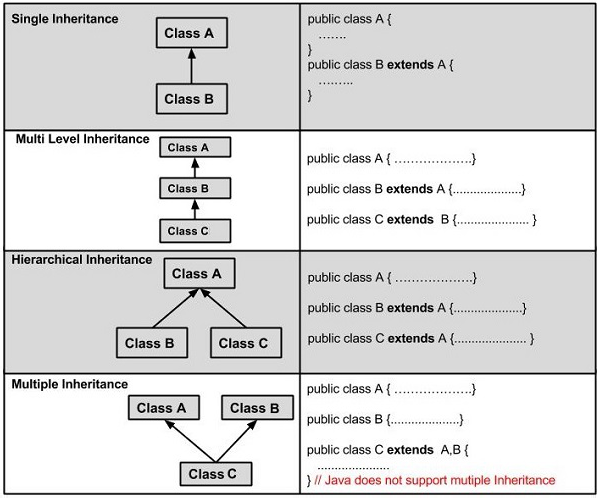
\includegraphics[width=6cm]{fig/types_of_inheritance.jpg}
    \caption{eksempel på typer af arv}
\end{figure}
\subsection{Forklar hvad abtract betyder}
Den abstrakte klasse kører ingen metoder, og indeholder kun attributter. Klassen bruges som en slags ”over”-klasse, hvor andre klasser nedarver attributterne. Det anvendes i en situation, hvor man f.eks har to klasser, der har mange af de samme attributter. Så vil alle de attributter, som de har tilfælles stå i den abstrakte klasse.
Hvis man f.eks har klasserne lærer og elev, kunne den abstrakte klasse til disse, hedde ”personer”, da både lærer og elever har en fødselsdato, køn, navn osv.

\subsection{Fortæl hvad det hedder hvis alle fieldklasserne har en landOnField metode der gør noget forskelligt}

% IOException: Sentence length out of bounds.
Hvis alle fieldklasserne gør brug af den samme landOnField metode, er det fordi, denne metode er en super metode. En super metode er nedarvet til de forskellige subklasser fra super klassen, dette gør at alle klasserne kan gøre brug af samme metode. Eksempeltvis, hvis vi har en masse dyr som klasser, kat, hund, kanin etc. så kan de alle nedarve super metoden eat() fra 
superklassen som hedder SurvivalRequirements, eftersom disse er metoder alle dyrene får brug for, så vil det give mening at lave det til en superklasse med supermetoder
, så der holdes lav kobling og høj kohæsion, samt undgås kopiring af kode og høj mulighed for genbrug.

\subsection{Dokumentation for test med screenshots}
    \subsection{JUnit test}
        JUnit test er en autonomisreret testmetode. Her skriver/koder man selv en test, som tester java kode. Oftest opbygger man JUnit test ud fra Java klasser.
        Der er mange måder, hvorpå man kan bruge JUnit testen. Man kan både skrive testen inden, man kan skrive den efter, man kan lave den på baggrund af indsigt i koden eller uden nogen form til kendskab af programkoden. Det to sidst nævnte kaldes Black- og Whitebox test.
        Her er et eksempel på et stykke udført JUnit test fra vores spil:
            \begin{figure}[h]\label{fig:JUnitTest} %FIGUR 7???
                \advance\leftskip-3cm
                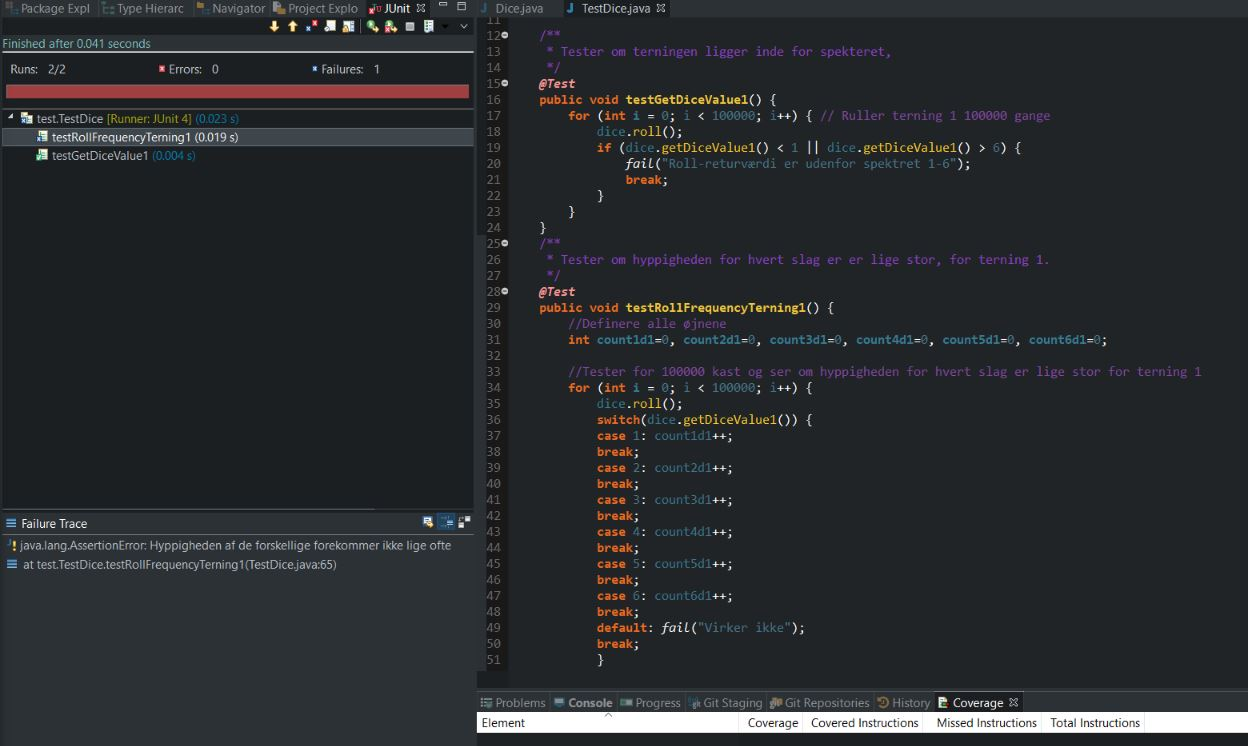
\includegraphics[width=20cm]{fig/JUnitTestDice.jpg}
                \caption{JUnit test udført i Eclipse den 23/11-2017}
            \end{figure}
        Det ser på Figur \ref{fig:JUnitTest} at koden ikke bestod testen, hvor vi også får vist den rette, selv skrevet, fejl besked.

    \subsection{Positiv negativ test}
        Denne test bruges for at teste om systemet kan håndterer 'ugyldige' input, dette kan både være negative som positive værdier, såvel som bogstaver og andre tegn. Denne test forbindes oftest med en eller flere ækvivalensklasse test.
    \subsection{Black- og Whitebox test}
        \textbf{Blackbox test}: Her har man intet kendskab til koden, ud over hvad denne skal kunne gøre. Det er derfor lige til højrebenet, at teste det faktiske output mod det forventede output og at teste ækvivalensklasserne.
        \\
        \textbf{Whitebox test}: Her opstiller man tests på baggrund af koden og dens opbygning. Man vil med disse tests teste hele koden, altså alle instruktioner, forgreninger og stier, som koden kan blive udført i. Dette er ikke altid muligt med \textit{BlackBox testen}, da man her, ikke har et indblik i koden.

\subsection{Dokumentation for overholdt GRASP}

\subsection{Vejledning til import af Git Repository til eclipse}
Man skal i første omgang have et URL af det pågældende repository, som du kopierer.
Derefter åbner du eclipse og åbner menuen 
Window $\Rightarrow$ View $\Rightarrow$ søg på "git" $\Rightarrow$ git repositories.
Derefter har du vinduet "Git Repositories", hvor der er en knap; "Clone a git repository and add to this view".
Ikonet er mappen i midten med en blå pil på, her trykker du.
Hvis du huskede at kopiere URL'et trykker du nu "Next", hvorefter at alle branches bliver loaded. Når den har loaded trykker du next igen.
Nu kommer du til det sidste vindue, hvor du trykker "Finish, og nu har du importeret(clonet) git repositoriet.

        \pagebreak
        %\input{test.tex}
    \end{document}